\section{Zeroth-Order Information: Neural Path Feature and Kernel}
\textbf{Paths:} We have a total of $P=d_{in}w^{(d-1)}$ paths. Let us say that an enumeration of the paths is given by $[P]=\{1,\ldots,P\}$. Let $\I_{l},l=0,\ldots,d-1$ provide the index of the hidden unit through which a path $p$ passes in layer $l$ (with the convention that $\I_d(p)=1,\forall p\in [P]$). We then define:\\
$1.$ The value of a path $p$ by $v_t(p)\stackrel{def}=\Pi_{l=1}^d \Theta_t(l,\I_{l-1}(p),\I_l(p))$.\\
$2.$ The activity of a path $p$ for an input $x\in \R^{d_{in}}$ by $A_{t}(x,p)\stackrel{def}{=}\Pi_{l=1}^{d-1} G_{x,t}(l,\I_l(p))$.\\
\begin{comment}
\FloatBarrier
\begin{table}[h]
\begin{minipage}{0.5\columnwidth}
\resizebox{\columnwidth}{!}{
\begin{tabular}{|c|l|}\hline								 								 													
NPF		&$\phi_{x,t}=(x(\I_0(p))A_t(x,p) ,p\in[P])\in \R^P$\\\hline	
OASN	&$\lambda_t(x,x')=\sum_{p\rsa i} A_t(x,p) A_t(x',p)$\\\hline
NPK		&$H_t(x,x')=\ip{\phi_{x,t},\phi_{x',t}}$\\\hline		
VTP		&$\varphi^v_{p,t}=(\partial_{\theta}v_t(p),\theta\in\Theta)\inrdnet$ \\\hline	
VG		&$\psi^v_{x,t}=\nabla_{\Theta} \hat{y}_t(x)\in\R^{d_{net}}$\\\hline
\end{tabular}
}
\end{minipage}
%\hspace{15pt}
\begin{minipage}{0.5\columnwidth}
\resizebox{\columnwidth}{!}{
\begin{tabular}{|c|l|}\hline								 								 													
ATP		&$\varphi^a_{x,p,t}=(\partial_{\tg}A_t(x,p),\tg\in\Tg)\inrdnet$ \\\hline	
FG		&$\psi^{\phi}_{x,t}=\nabla_{\Tg} \hat{y}_t(x)\in\R^{d_{net}}$\\\hline
OSSN 	&$\delta_t(x,x')=\sum_{p\rsa i} \ip{\varphi^a_{x,p,t},\varphi^a_{x',p,t}}$\\\hline
NTF		&$\psi_{x,t}=(\psi^v_{x,t},\psi^{\phi}_{x,t})\in\R^{2d_{net}}$\\\hline
NTK 		&$K_t(x,x')=\ip{\psi_{x,t}\psi_{x',t}}$\\\hline
\end{tabular}
}
\end{minipage}
\caption{Shows all zeroth-order and first-order quantities related to information flow in a DGN.}
\label{tb:terms}
\end{table}
\end{comment}
The \textbf{neural path feature (NPF)} of an input example $x_s\in \R^{d_{in}}$ is given by $\phi_{x_s,\G_t}=(x_s(\I_0(p))A_t(x_s,p) ,p\in[P])\in\R^P$. Here, for a path $p$, $\I_0(p)$ is the input node at which the path starts and $A_t(x_s,p)$ is its activation level. By arranging the NPF of the $n$ input examples in a matrix $\Phi_t=(\phi_{x_s,\G_t},s\in[n)\in\R^{P\times n}$, we can express the predicted output of a DGN as: 
\begin{align}\label{eq:npfbasic}
\hat{y}_t=\Phi_t^\top v_t,
\end{align}
where, the value of the path $v_t$ is the equivalent of the so called \emph{weight-vector} in a standard linear approximation. 
The significance of the NPF is that it separates the \emph{signal} form the \emph{wire}. Note that $\Phi$ encodes the signal: say for a DNN with ReLU activations, the co-ordinate corresponding to path $p$ is either $x(\I_0(p))$ if the path is active for that input (i.e., $A_t(x,p)=1$) or $0$ if the path is inactive for that input  (i.e., $A_t(x,p)=0$). The value of the path encodes the \emph{wire}, i.e., the information contained in the weights of the network.
% \textbf{Active Sub-Network:}  For input $x_s\in\R^{d_{in}}$, let $\N^{\A}_{x_s,t}(\tau_{\A})=\{p\in[P]:A_t(x,p)>\tau_{\A}\}$ be the \emph{active sub-network} comprising of the set of paths whose activity is greater than some threshold value $\tau_{\A}>0$. In the case of ReLU activations, $\N^{\A}_{x_s,t}(0)$ completely determines the NPF $\phi_{x_s,\G_t}$.  $\lambda_t(x_s,x_{s'})$ is a measure of overlap of active sub-networks for input examples $s,s'\in[n]$.
\begin{lemma}\label{lm:npk}
Let $\lambda_t(s,s')\stackrel{def}{=}\sum_{p\rsa i} A_t(x_s,p) A_t(x_{s'},p)$, $\forall s,s'\in[n]$, any $i\in [d_{in}]$ and let the \textbf{neural path kernel} (NPK) matrix is defined as $H_t\stackrel{def}=\Phi^\top_t\Phi_t$. It follows that $H_t= (x^\top x')\odot\lambda_t$. 
\end{lemma}
From \Cref{lm:npk} it follows that the similarity of two inputs $s,s'\in[n]$ is depends on $\ip{x_s,x_{s'}}$, and the overlap of the active paths for those inputs captured by $\lambda_t(s,s')$.\\
\section{Learning with Neural Path Features}
\begin{comment}
\textbf{NPFs and Optimisation:} The ability of DNNs to fit data has been demonstrated in the past \cite{ben}, i.e., they can fit even random labels, and random pixels of standard datasets such as MNIST. However, for standard DNNs with ReLU gates, with no bias parameters, a dataset with $n=2$ points namely $(x,1)$ and $(2x,-1)$ for some $x\in \R^{d_{in}}$ cannot be memorised. The reason is that the gating values are the same for both $x$ and $2x$ (for that matter any positive scaling of $x$), and hence $\phi_{2x,\G_t }= 2\phi_{x,\G_t }$, and thus it not possible to fit arbitrary values for $\hat{y}_t(x)$ and $\hat{y}_t(2x)$.\\
\end{comment}
 We trained DGN on standard datasets namely MNIST and CIFAR-10, under the following conditions: i) the gates are frozen $\G_t=\G_0,\forall t\geq 0$ and ii) the gating values are obtained from a ReLU network, which acts as the gating network (see \Cref{tb:dgn}). Since, the gates are frozen, the NPFs are fixed and the SGD learns only the path values. We compare the performance of $4$ different NPFs, wherein, the gates are copied from i) from a randomly initialised ReLU network (untrained), ii) from a ReLU network trained with good dataset iii) ReLU network trained on random labels and iv) ReLU network trained on random pixels.
\FloatBarrier
\begin{table}[h]
\begin{tabular}{|c|c|c|c|c|c|c|}\hline
&&&&\multicolumn{3}{c|}{NPF (trained)}\\\cline{5-7}
$(w,d)$	&Dataset		&ReLU		&NPF(untrained) 		&Good 		&Random Labels 	&Random Pixel\\\hline
$(128,6)$	& MNIST 		& $98.15$ 		&$96$ 		&$98.3$		&$92.6$			&$94.3$\\\hline
$(256,6)$	& MNIST 		& $98.5$ 		&$96.6$ 		&$98.4$		&$92.0$			&$81.1$\\\hline
\end{tabular}
\caption{Shows the training and generalisation performance of various GaLU network. Here, non-learned stands for gates from a randomly initialised ReLU network.}
\label{tb:npfs}
\end{table}
\FloatBarrier
\begin{wrapfigure}{h}{0.3\textwidth}
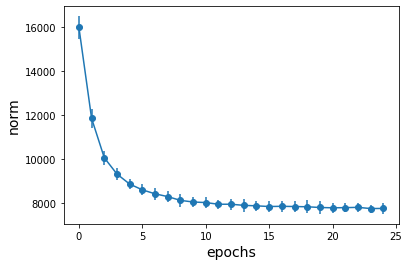
\includegraphics[scale=0.25]{figs/path-gram.png}
\caption{\label{fig:frog1}This is a figure caption.}
\end{wrapfigure}
\textbf{NPF dynamics:} We consider ``Binary''-MNIST data set with two classes namely digits $4$ and $7$, with the labels taking values in $\{-1,+1\}$ and squared loss. We trained a standard DNN with ReLU activation ($w=100$, $d=5$). Recall that $H_t=\Phi^\top_t\Phi_t$  (the Gram matrix of the features) and let $\widehat{H}_t=\frac{1}{trace(H_t)}H_t$ be its normalised counterpart. For a subset size, $n'=200$ ($100$ examples per class) we plot $\nu_t=y^\top (\widehat{H}_t)^{-1} y$, (where $y\in\{-1,1\}^{200}$ is the labeling function), and observe that $\nu_t$ reduces as training proceeds (see first plot in \Cref{fig:gen}). Note that $\nu_t=\sum_{i=1}^{n'}(u_{i,t}^\top y)^2 (\hat{\rho}_{i,t})^{-1}$, where $u_{i,t}\in \R^{n'}$ are the orthonormal eigenvectors of $\widehat{H}_t$ and $\hat{\rho}_{i,t},i\in[n']$ are the corresponding eigenvalues. Since $\sum_{i=1}^{n'}\hat{\rho}_{i,t}=1$, the only way $\nu_t$ reduces is when more and more energy gets concentrated on $\hat{\rho}_{i,t}$s for which $(u_{i,t}^\top y)^2$s are also high. However, in $H_t=(x^\top x)\odot \lambda_t$, only $\lambda_t$ changes with time. Thus, $\lambda_t(s,s')$ which is a measure of overlap of sub-networks active for input examples $s,s'\in[n]$, changes in a manner to reduce $\nu_t$. We can thus infer that the \emph{right} active sub-networks are learned over the course of training. We now summarise the insights obtained from these experiments in the following remarks:\hfill\\

\section{First-Order Information: Neural Tangent Feature and Kernel}
Consider a DGN, wherein, the gating network is parameterised by $\Tg\inrdnet$ with $\beta>0$.  We have 
\begin{align}\nabla_{\Theta,\Tg}\hat{y}_t=\psi_{x,t}=(\psi^v_{x,t}, \psi^{\phi}_{x,t})=\left((\nabla_{\Theta|_{\Theta=\Theta_t}}v_{\Theta})^\top \Phi_{\Tg_t}, (\nabla_{\Tg|_{\Tg=\Tg_t}}\Phi_{\Tg_t})^\top v_{\Theta_t}\right)\in \R^{2d_{net}}
\end{align}
$1.$ The \emph{value gradient}  $\psi^v_{x,t}$ flows through the network of active paths: For a path $p$, the derivative of its value with respect to any weight in the path is given by:\\
\begin{align}\label{eq:vft}{\partial v_t(p)}/{\partial \Theta\left(l,\I_{l'-1}(p),\I_{l'}(p)\right)}|_{\Theta=\Theta_t}= \underset{l=1}{\underset{l\neq l'}{\overset{d}{\Pi}}} \Theta_t\left(l,\I_{l-1}(p),\I_{l}(p)\right)
\end{align}
Note that, if a path $p$ does not pass through a $\theta\in\Theta$, then ${\partial v_t(p)}/{\partial \theta}=0$. Further, since $\psi^v_{x,t}=(\nabla_{\Theta|_{\Theta=\Theta_t}}v_{\Theta})^\top \Phi_{\Tg_t}$, the value derivatives of those paths which are not active, i.e., $A_t(x_s,p)$ close to $0$ will not be counted in $\psi^v_{x,t}$.\\
$2.$ The \emph{feature gradient}  $\psi^{\phi}_{x,t}$ flows through the network of sensitive paths: Note that for a weight $\tg\in \Tg$, $\partial_{\tg} \phi_{x_s,t}(p) = x(\I_0(p))\partial_{\tg} A_t(x_s,p)$, wherein,:\\
\begin{align}
\frac{\partial A_{t}(x,p)}{\partial \tg}= \sum_{l=1}^{d-1} \Big(\frac{\partial G_{x,\Tg_t}(l,\I_l(p))}{\partial \tg} \Big)\Big(\Pi_{l'\neq l} G_{x,\Tg_t}(l',I_{l'}(p))\Big)
\end{align}
Note that if all the activations in a path are close to $0$ or $1$, then $\partial_{\tg} A_t(x_s,p)$ is close to $0$.\\
$3.$ Let $\N^{\A}_{x_s,t}(\tau_{\A})=\{p\in[P]:A_t(x,p)>\tau_{\A}\}$ be the \emph{active sub-network} comprising of the set of paths whose activity is greater than some threshold value $\tau_{\A}>0$. Let $\N^{\S}_{x,t}(\tau_{\S})=\{p\in[P]: |\partial_{\tg} A_t(x,p)|>\tau_{\S}\}$ be sensitive sub-network, whose path activity gradient with respect to any of $\Tg\inrdnet$ is greater than some threshold $\tau_{\S}>0$. Using the property that the slope of the sigmoid diminishes in the extremities, we can reason that for appropriate choices of $\tau_{\A}$ (sufficiently close to $1$) and $\tau_{\S}$ (large enough), $\P^{\S}(\tau_{S})\cup \P^{\A}(\tau_{\A})=\emptyset$. Thus, there are two separate networks for the two separate gradient flows, i.e., the value gradient flow via the active sub-network and the feature gradient flow via the sensitive sub-network.\\
%$4.$ In the case when the parameters are shared, i.e., $\Tg=\Theta$, we have $\nabla_{\Theta}\hat{y}_t=\psi^v_{x,t}+ \psi^{\phi}_{x,t}$.\\
$4.$ In the case of $\beta=\infty$ (see \Cref{tb:dgn}), i.e, when the gating values belong to $\{0,1\}$, it follows that the activity $A_t\in\{0,1\}$ and hence $\partial_{\tg} A_t(\cdot,\cdot)=0$. Thus, in the case of DNNs with ReLU activations, there is no flow of the feature gradient, however, since the gating parameter $\Tg$ identical with $\Theta$, (i.e., $\Tg_t=\Theta_t,\forall t$), $A_t$ changes with time and so does the NPF. \\
\begin{comment}
\begin{definition}\label{def:delta}
$\delta_t(s,s')=\sum_{p\rsa i} \ip{\varphi^a_{x_s,p,t},\varphi^a_{x_{s'},p,t}}$, for $s,s'\in[n]$, using any $i\in[d_{in}]$.
\end{definition}
\textbf{Gradient Flow via Sub-Networks:} Note that in the case of $\beta=\infty$ (see \Cref{tb:dgn}), i.e, when the gating values belong to $\{0,1\}$, it follows that the activity $A_t\in\{0,1\}$, and hence AD and FG are $0$. Thus, in the case of DNNs with ReLU activations, there is no flow of the feature gradient, however, since the gating parameter $\Tg$ identical with $\Theta$, (i.e., $\Tg_t=\Theta_t,\forall t$), $A_t$ changes with time and so does the NPF. In the case of $\beta>0$, for an input $x\in\R^{d_{in}}$, let $\N^{\S}_{x,t}(\tau_{\S})=\{p\in[P]: |\partial_{\tg} A_t(x,p)|>\tau_{\S}\}$ be the set of paths, which have activations whose gradient to any of $\Tg\inrdnet$ is greater than some threshold $\tau>0$. Note that when all the gates are close to $1$ in a path $p$, then it follows that $\partial A_t(x_s,p)$ will be very small. Thus, using the property that the slope of the sigmoid diminishes in the extremities, we can reason that for appropriate choices of $\tau_{\A}$ (sufficiently close to $1$) and $\tau_{\S}$ (large enough), $\P^{\S}(\tau_{S})\cup \P^{\A}(\tau_{\A})=\emptyset$. Thus, there are two separate networks for the two separate gradient flows, i.e., the value gradient flow via the active sub-network and the feature gradient flow via the sensitive sub-network.\\
\end{comment}
\begin{assumption}\label{assmp:init}
The weights $\Theta_0$ are sampled i.i.d from a distribution such that for any $\theta_0\in\{\Theta_0\cup \Tg_0\}$,  we have $\E{\theta_0}=0$, and  $\E{\theta^2_0}=\sigma^2$, and $\E{\theta^4_0}={\sigma'}^2$.
\end{assumption}
\begin{lemma}\label{lm:disentangle}[Disentanglement] Let $\varphi_{p,t}=\nabla_{\Theta} v_t(p)\inrdnet$, 
under \Cref{assmp:init}, $\forall\,\theta\in\Theta$, for paths $p,p'\in [P], p\neq p'$:  i) $\E{\ip{\varphi_{p,0},\varphi_{p',0}}}= 0$ and ii)$\E{\ip{\varphi_{p,0},\varphi_{p,0}}}= \sigma^{2(d-1)}$, iii) $\E{v_0(p)v_0(p')}=0$, iv) $\E{v^2_0(p)}=\sigma^{2d}$.
\end{lemma}
\textbf{Neural Tangent Feature and Kernel:} Let $\Psi^v_t=(\psi^v_{x_s,t},s\in[n])\in\R^{d_{net}\times n}$ and $\Psi^{\phi}_t=(\psi^{\phi}_{x_s,t},s\in[n])\in\R^{d_{net}\times n}$ be the NTF matrices, then the corresponding NTK matrices are given in \Cref{tb:ntks}
\FloatBarrier
\begin{table}[h]
\begin{minipage}{0.5\columnwidth}
%\resizebox{\columnwidth}{!}{
\begin{tabular}{|c|l|}\hline								 								 													
NTF		&$\psi_{x_s,t}=(\psi^v_{x_s,t},\psi^{\phi}_{x_s,t})\in\R^{2d_{net}}$\\\hline
NTK 		&$K_t=K^v_t+K^{\phi}_t$\\\hline
\end{tabular}
%}
\end{minipage}
%\hspace{15pt}
\begin{minipage}{0.5\columnwidth}
%\resizebox{\columnwidth}{!}{
\begin{tabular}{|c|l|}\hline								 								 													
NTF		&$\psi_{x_s,t}=(\phi^v_{x_s,t}+\psi^{\phi}_{x_s,t})\in\R^{d_{net}}$\\\hline
NTK 		&$K_t=K^v_t+K^{\phi}_t+{\Psi^{\phi}}^\top_t\Psi^v_t+ {\Psi^{v}}^\top_t\Psi^{\phi}_t$\\\hline
\end{tabular}
%}
\end{minipage}
\caption{Shows NTK and NTF for the distinct ($\Tg\neq\Theta$) on the left and shared parameterisation ($\Tg=\Theta$) on the right. Here, $K^v_t={\Psi^{v}}^\top_t\Psi^v_t$ and $K^{\phi}_t={\Psi^{\phi}}^\top_t\Psi^{\phi}_t$.}
\label{tb:ntks}
\end{table}

\begin{comment}
The \textbf{neural tangent feature} (NTF) is given by $\psi_{x_s,t}=(\psi^v_{x_s,t},\psi^{\phi}_{x_s,t})\in\R^{2d_{net}}$, when the gating network is parameterised by $\Tg$ which is distinct from $\Theta$. When the parameters are shared ($\Tg_t=\Theta_t\forall t\geq 0$), then we have $\psi_{x_s,t}=(\phi^v_{x_s,t}+\psi^{\phi}_{x_s,t})\in\R^{d_{net}}$.\\
When the gating network is parameterised by $\Tg$ which is distinct from $\Theta$, the \textbf{neural tangent kernel} (NTK) matrix is given by $K_t=K^v_t+K^{\phi}_t$, where $K^v_t={\Psi^{v}}^\top_t\Psi^v_t$ and $K^{\phi}_t={\Psi^{\phi}}^\top_t\Psi^{\phi}_t$, with $\Psi^v_t=(\psi^v_{x_s,t},s\in[n])\in\R^{d_{net}\times n}$ and $\Psi^{\phi}_t=(\psi^{\phi}_{x_s,t},s\in[n])\in\R^{d_{net}\times n}$. In the case of shared parameterisation ($\Tg_t=\Theta_t\forall t\geq 0$), we have $K_t=K^v_t+K^{\phi}_t+{\Psi^{\phi}}^\top_t\Psi^v_t+ {\Psi^{v}}^\top_t\Psi^{\phi}_t$.
\end{comment}